\chapter{Ergebnisse}
Im Rahmen dieses Projektes wurde ein Control-Panel entwickelt, das in der Lage ist,
mit einem Smarthome zu kommunizieren. Das Control-Panel ist in der Lage,
Sensor-Daten zu empfangen sowie die relevanten IP und MAC-Adressen des Smarthomes
anzuzeigen. Das Menu des Control-Panels kann über einen Rotary Encoder gesteuert
werden.\\

Es wurde eine funktionsfähige Platine entwickelt und ein Gehäuse
konstruiert, das alle Komponenten des Control-Panels enthält. Die Ausgabe am Display
sowie die Eingabe über den Encoder funktionieren. Es können die ARGB-LEDs angesteuert werden
und ein Ton über den Piezo ausgegeben werden. \\~\\


% \begin{figure}[htbp]
%     \centering
%     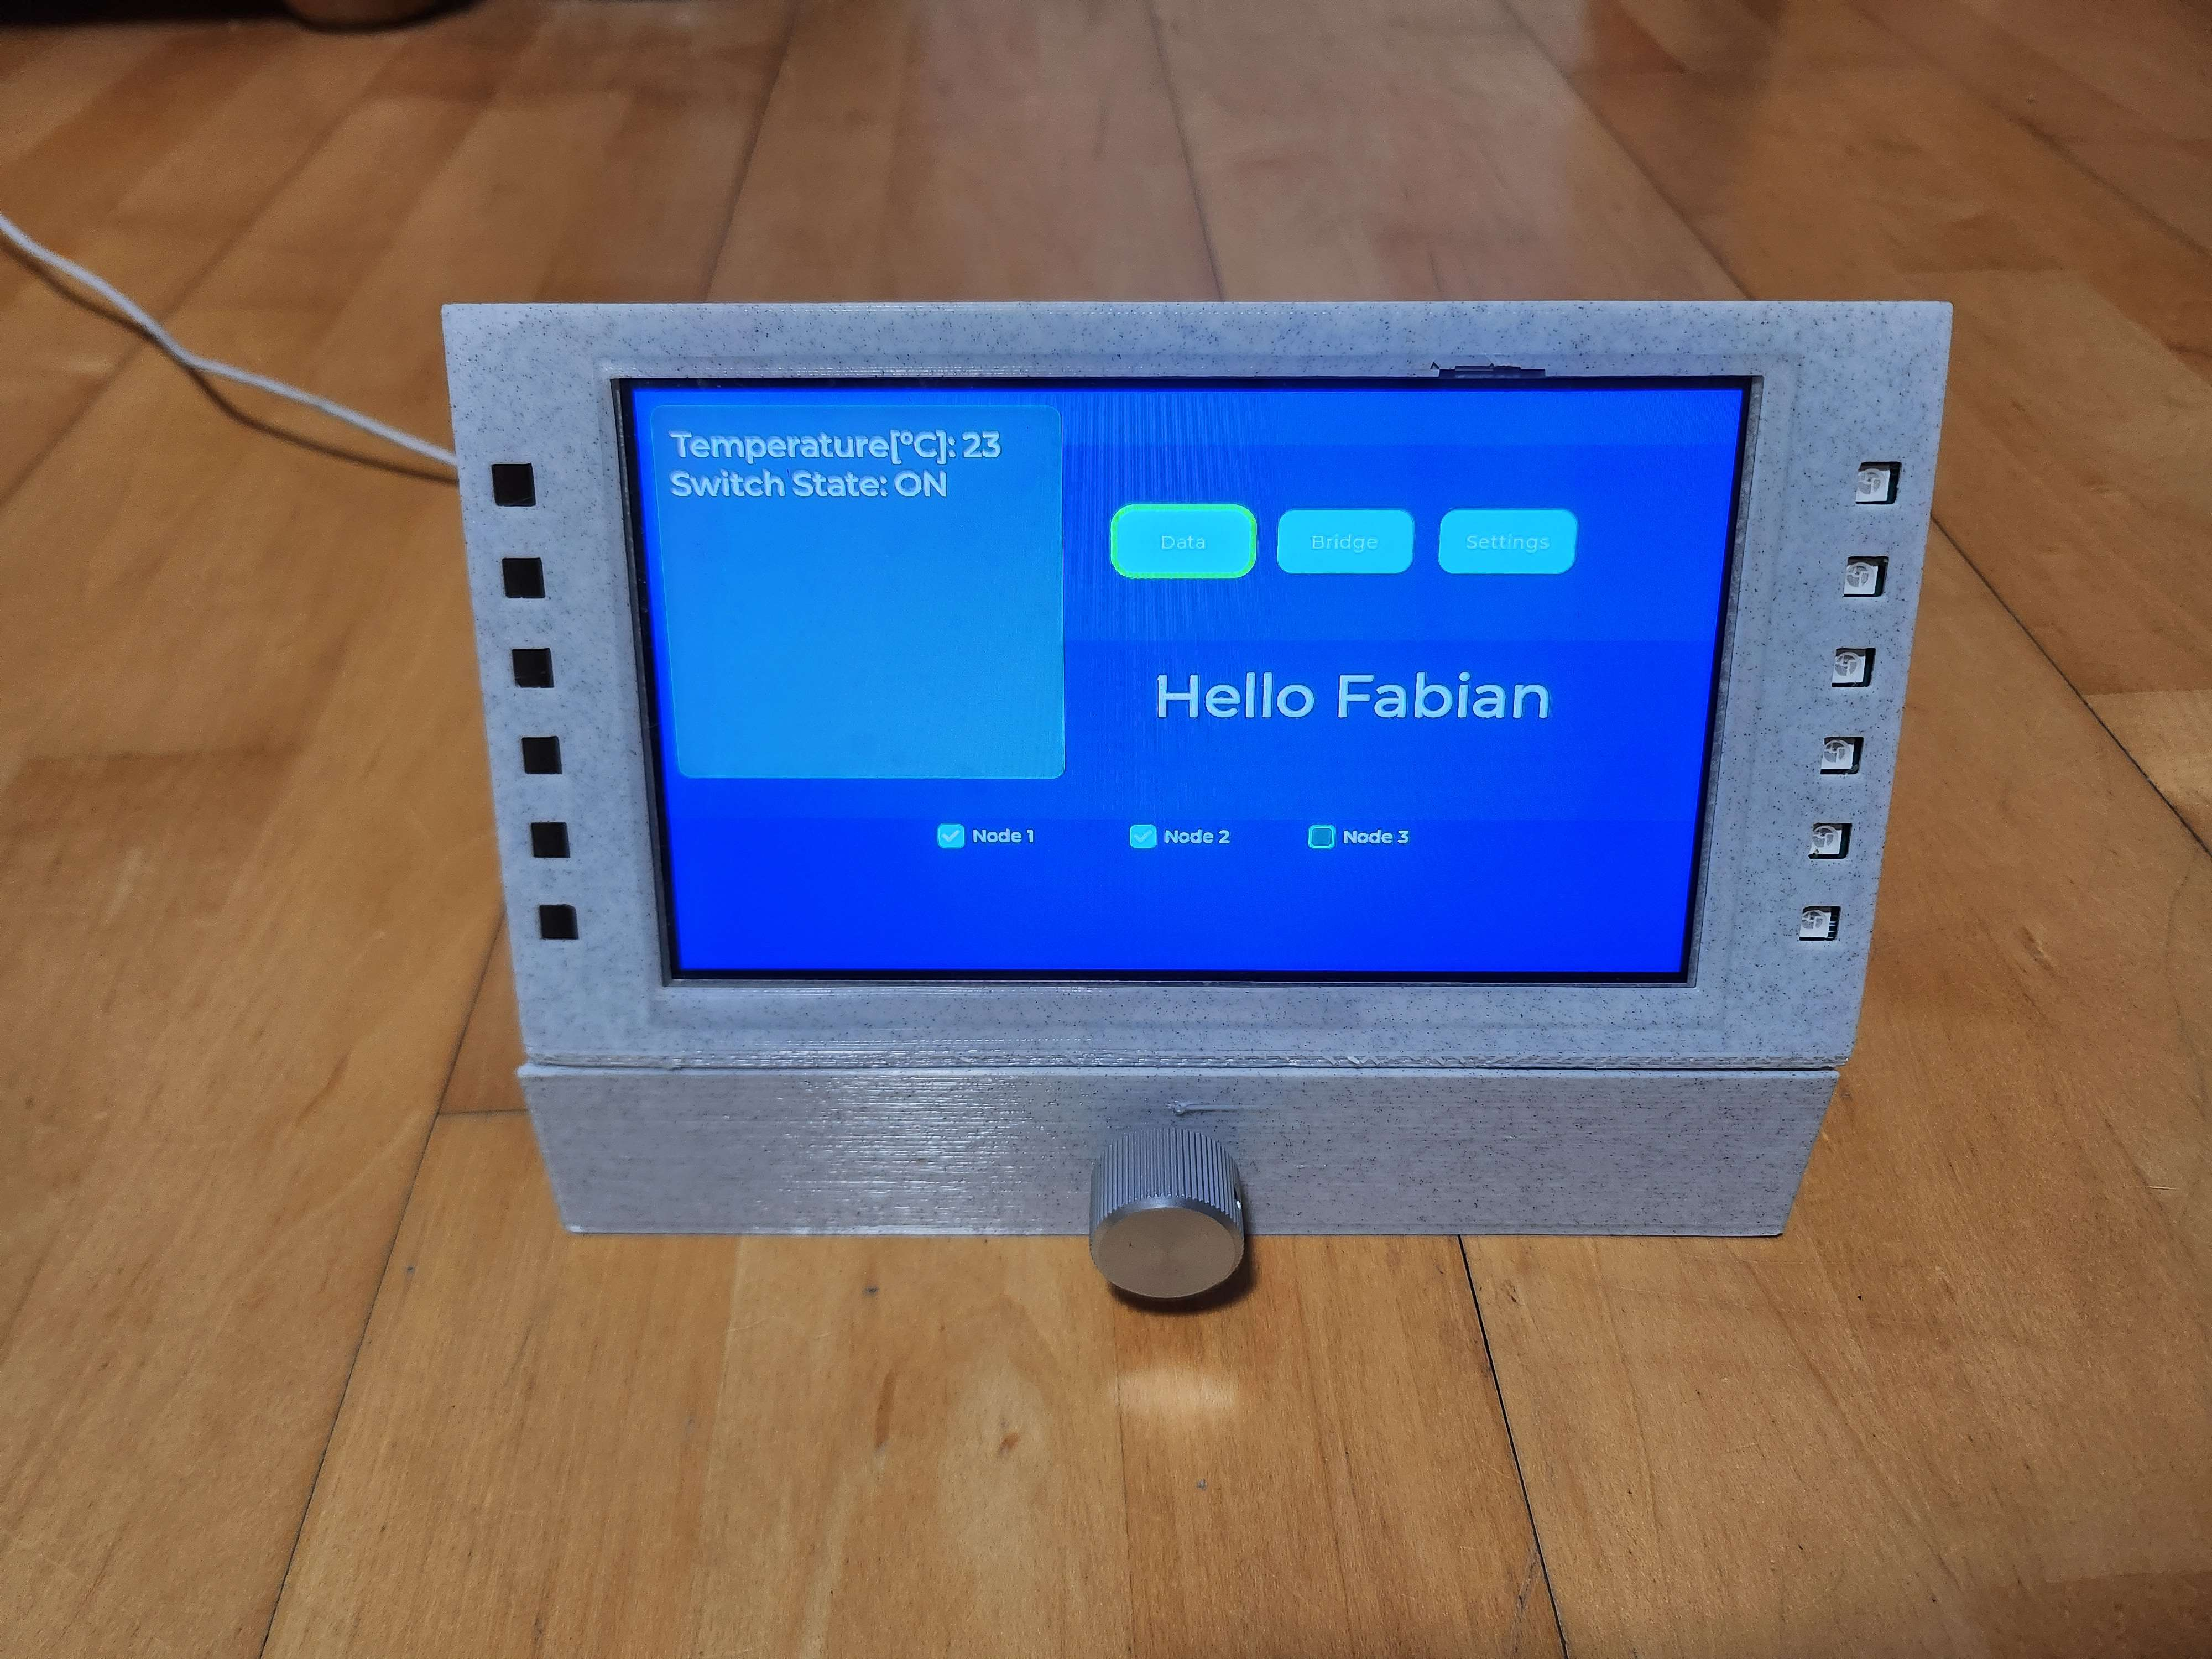
\includegraphics[width=0.8\textwidth]{assets/ControlPanel.jpg}
%     \caption{Control-Panel}
%     \label{fig:control-panel}
% \end{figure}
